In this section, we provide a brief overview of \oursystem architecture as shown in Figure~\ref{overview}. \oursystem firstly builds up reference point database which stores the geographical information of reference points together with vision descriptors extracted by the site survey component. When a user sends query feature points extracted by the querier component to the server, the search component finds the nearest neighbors of query features by two-stage search scheme. At last, the localization component inversely calculates the user's location and sends the result to the user.
\begin{figure}[!ht]
\centering
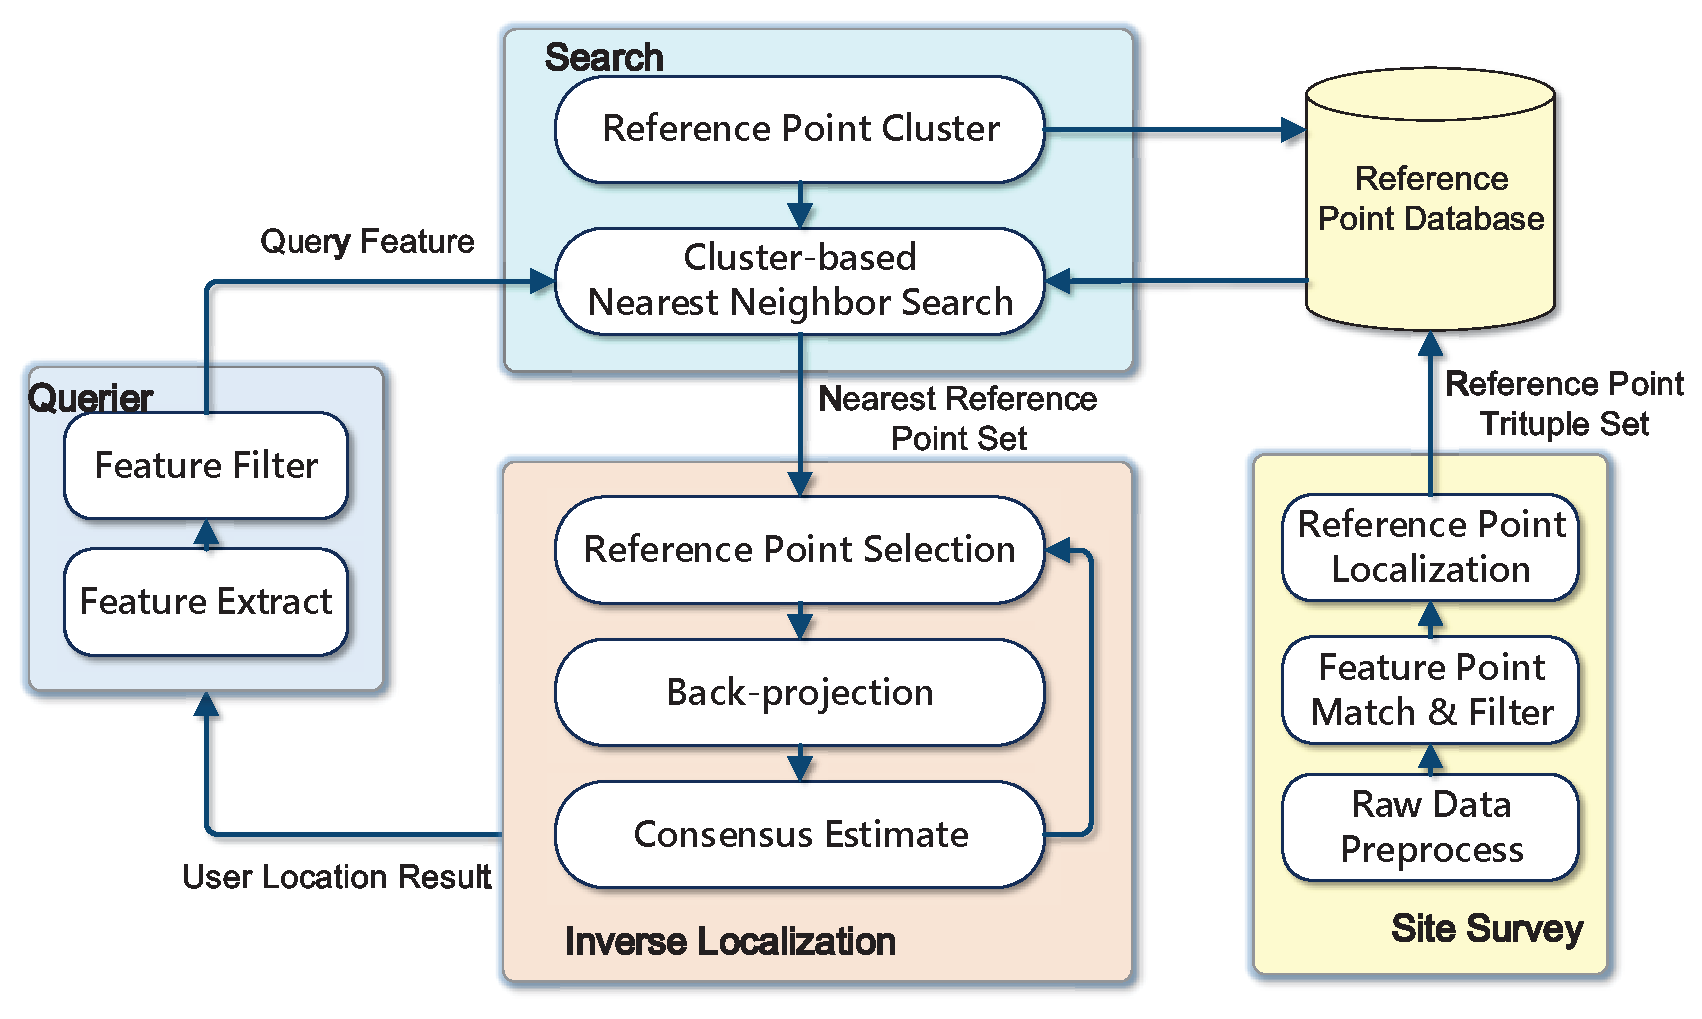
\includegraphics[width=1\linewidth, clip,keepaspectratio]{overview2.eps}
\caption{\oursystem system architecture.}\label{overview}
\end{figure}


\oursystem consists of four components:


\textbf{(1)Querier Component:}
This component runs on smartphone as an application for users. It extracts the feature points from the query photo taken by a user, and generates a descriptor for each feature point. But we don't need all feature points, for the reason of saving communication cost and filtering out the unstable feature points, \ie features not on building structures or features on people, which would decrease accuracy of localization.

\textbf{(2)Site Survey Component:}
Site survey component builds up the specific reference point database for a building. We calculate the geographical location of a reference point according to its depth which is figured out by binocular ranging. Binocular ranging makes use of the disparity of one feature point to calculate its depth. In order to obtain the disparity of feature points, we firstly take pair-photos(Figure~\ref{pair}) for the building on the predefined survey track. Then this component extracts feature points from pair-photos. It matches the feature point in the left photo to the most similar feature point in the right photo to calculate disparity of this feature. However, some matches are not similar enough or not reasonable, \eg one feature on the floor matches to one on the ceiling though their descriptors are similar. These bad matches should be thrown away because they may impact the calculation of geographical position of reference point. Then we indicate the geographical coordinates of feature point according to its depth and pixel coordinates. We combine the descriptor of a feature point with its geographical coordinates to form a reference point and store all of them into reference point database.

\textbf{(3)Search Component:}
\begin{figure}[t!]
\centering
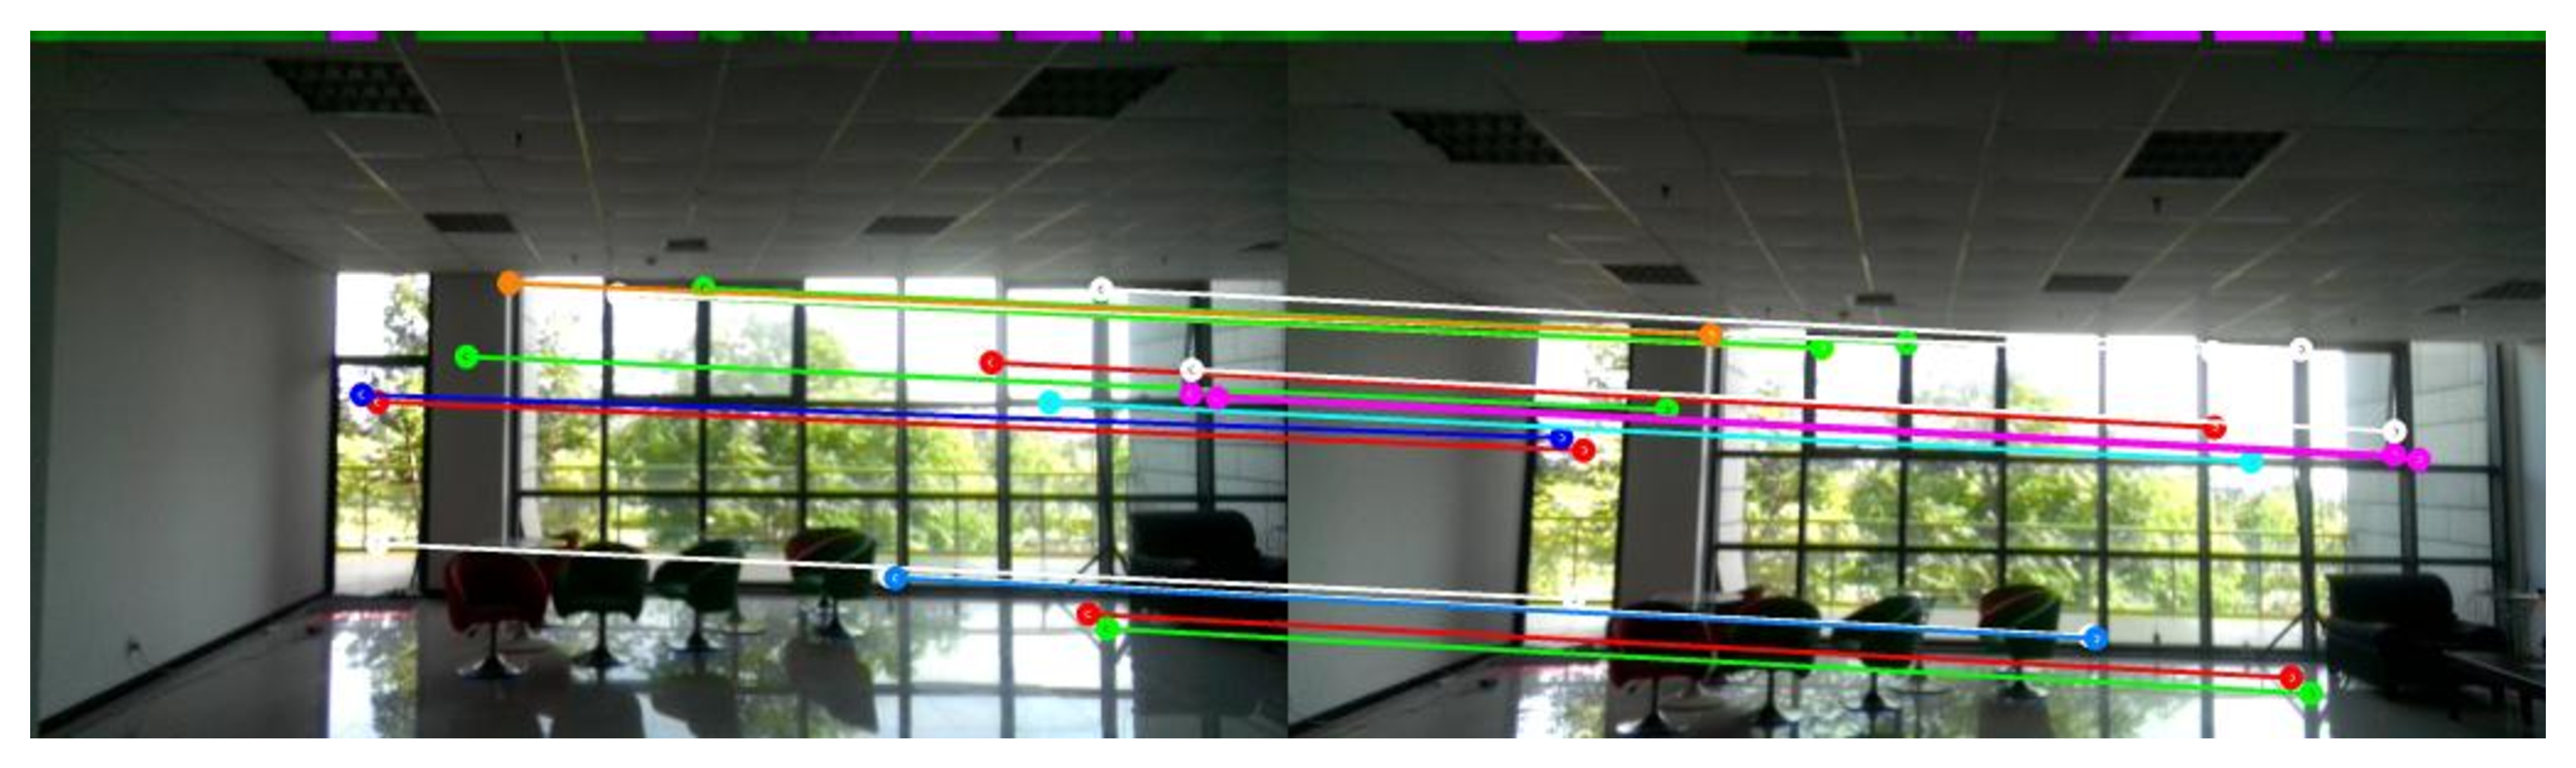
\includegraphics[width=1\linewidth, clip,keepaspectratio]{pair_photo.eps}
\caption{Pair-photo with feature point matches.}\label{pair}
\end{figure}
Given a localization request, the search module will find the nearest neighbor for each query feature descriptor using two-stage cluster-based search algorithm. The cluster-based search algorithm makes use of feature point clusters generated by reference point cluster component. One cluster consists of reference points whose feature descriptors are near to each other in Euclidean distance. In one cluster, we choose a reference point to represent all points in it and this representative can be treated as the centroid of cluster.

\textbf{(4)Inverse Localization Component:}
This component inversely calculates user's location as soon as the search component outputs the nearest neighbor set of query feature points. Firstly, we choose the trine of match from search component's outputs. Each trine contains three matches between query points and reference points. We sort these trines according to the similarity of matches measured by the distance between two feature points. The trine whose matches have high similarity will get high priority. We calculate the geographical location of user by solving the location determination problem(LDP). As we figure out a location, we estimate the error of location by calculating the consensus of it in its nearest neighbor set. The location with low consensus is possible to be inaccurate, so we discard it and start another round of inverse calculation. This process stops until the number of rounds exceeds the threshold. At last, this component returns the most accurate result of user's location.
